%%%%%% -*- Coding: utf-8-unix; Mode: latex

\documentclass[polish]{projectreport}

\usepackage[utf8]{inputenc}
\usepackage{url}
\usepackage{subfigure}
\usepackage{tabularx}
\usepackage{ragged2e}
\usepackage{booktabs}
\usepackage{multirow}
\usepackage{grffile}
\usepackage{float}

\usepackage[bookmarks=false]{hyperref}
\hypersetup{colorlinks,
  linkcolor=blue,
  citecolor=blue,
  urlcolor=blue}

\usepackage{indentfirst}
\usepackage{caption}
\usepackage{listings}
\usepackage[ruled,linesnumbered,lined]{algorithm2e}
\usepackage[svgnames]{xcolor}
\usepackage{inconsolata}
\usepackage{fancyhdr}
\usepackage{microtype} 

\usepackage{csquotes}
\DeclareQuoteStyle[quotes]{polish}
  {\quotedblbase}
  {\textquotedblright}
  [0.05em]
  {\quotesinglbase}
  {\fixligatures\textquoteright}
\DeclareQuoteAlias[quotes]{polish}{polish}

\usepackage[
style=numeric,
sorting=nyt,
isbn=false,
doi=true,
url=true,
backref=false,
backrefstyle=none,
maxnames=10,
giveninits=true,
abbreviate=true,
defernumbers=false,
backend=biber]{biblatex}
\addbibresource{bibliography.bib}

\lstset{
    basicstyle=\ttfamily\footnotesize,
    backgroundcolor=\color{gray!5},
    commentstyle=\it\color{Green},
    keywordstyle=\color{Red},
    stringstyle=\color{Blue},
    numberstyle=\tiny\color{Black},
    escapeinside=`',
    frame=single,
    tabsize=2,
    rulecolor=\color{black!80},
    title=\lstname,
    breaklines=true,
    breakatwhitespace=true,
    framextopmargin=2pt,
    framexbottommargin=2pt,
    extendedchars=false,
    captionpos=b,
    abovecaptionskip=5pt,
    keepspaces=true,
    numbers=left,
    numbersep=5pt,
    showspaces=false,
    showstringspaces=false,
    showtabs=false,
    tabsize=2
}

\SetAlgorithmName{\LangAlgorithm}{\LangAlgorithmRef}{\LangListOfAlgorithms}

\renewcommand{\lstlistingname}{\LangListing}
\renewcommand\lstlistlistingname{\LangListOfListings}

\newcolumntype{Y}{>{\small\centering\arraybackslash}X}

\captionsetup[figure]{skip=5pt,position=bottom}
\captionsetup[table]{skip=5pt,position=top}


%%%%%%%%%%%%%%%%%%%%%%%%%%%%%%%%%%%%%%%%%%%%%%%%%%%%%%%%%%%%%%%%%%%%%%%%%%%%%%%
\author{Dawid Czesak \and Dominik Matras}

\title{Symulacja prostego systemu spo{\l}eczno-ekonomicznego}

\date{
    {\small \texttt{dczesak@student.wszib.edu.pl}\\[1ex]
    \texttt{dmatras@student.wszib.edu.pl}\\[2ex]
    \texttt{\href{https://github.com/dominikmatras/latex_miss_project}{github.com/dominikmatras/latex\_miss\_project}}\\[2ex]
    \the\year}
}

\pagestyle{fancy}
\fancyhf{}
\fancyhead[LE,RO]{\thepage}

%%%%%%%%%%%%%%%%%%%%%%%%%%%%%%%%%%%%%%%%%%%%%%%%%%%%%%%%%%%%%%%%%%%%%%%%%%%%%%%
\begin{document}

\maketitle

\thispagestyle{empty}

\begin{abstract}
\noindent
Niniejsza praca przedstawia projekt oraz analiz\k{e} prostej symulacji systemu
spo\l{}eczno-\allowbreak ekonomicznego opartej na modelu agentowym (\emph{Agent-Based Modeling}, ABM).
W~opracowanym modelu populacja stu agent\'ow reprezentuje uczestnik\'ow systemu
ekonomicznego, kt\'orzy posiadaj\k{a} okre\'slony maj\k{a}tek pocz\k{a}tkowy, uzyskuj\k{a} losowy
doch\'od, ponosz\k{a} koszty utrzymania oraz uczestnicz\k{a} w~losowych transakcjach
finansowych. Symulacj\k{e} przeprowadzono w~trzech wariantach r\'o\.{z}ni\k{a}cych si\k{e}
poziomem redystrybucji maj\k{a}tku: 0\%, 5\% oraz 10\%. Wyniki eksperyment\'ow
pokazuj\k{a}, \.{z}e nawet w~uproszczonym systemie, w~kt\'orym wszyscy agenci startuj\k{a}
z~identycznym maj\k{a}tkiem, po pewnym czasie pojawiaj\k{a} si\k{e} nier\'owno\'sci maj\k{a}tkowe.
Zastosowanie mechanizmu redystrybucji skutecznie ogranicza narastanie tych
nier\'owno\'sci, mierzone wsp\'o\l{}czynnikiem Giniego, nie zmieniaj\k{a}c przy tym
\'sredniego maj\k{a}tku ca\l{}ej populacji. Praca pokazuje, \.{z}e modelowanie agentowe
mo\.{z}e stanowi\'{c} u\.{z}yteczne narz\k{e}dzie do analizy podstawowych mechanizm\'ow
spo\l{}eczno-\allowbreak ekonomicznych, takich jak powstawanie nier\'owno\'sci i~wp\l{}yw
redystrybucji na struktur\k{e} maj\k{a}tkow\k{a} populacji.
 
\medskip
\noindent\textbf{S\l{}owa kluczowe:} symulacja wieloagentowa, systemy spo\l{}eczno-ekonomiczne,
nier\'owno\'sci maj\k{a}tkowe, redystrybucja, wsp\'o\l{}czynnik Giniego, modelowanie agentowe
\end{abstract}

%%%%%%%%%%%%%%%%%%%%%%%%%%%%%%%%%%%%%%%%%%%%%%%%%%%%%%%%%%%%%%%%%%%%%%%%%%%%%%%
\section{\SectionTitleIntroduction}
\label{sec:introduction}

%%%%%%%%%%%%%%%%%%%%%%%%%%%%%%%%%%%%%%%%%%%%%%%%%%%%%%%%%%%%%%%%%%%%%%%%%%%%%%%
\subsection{Wprowadzenie}
\label{sec:intro}

Systemy spo\l{}eczno-ekonomiczne s\k{a} z\l{}o\.{z}onymi uk\l{}adami, w~kt\'orych wiele jednostek podejmuje
decyzje dotycz\k{a}ce pracy, konsumpcji, oszcz\k{e}dzania, wymiany d\'obr oraz korzystania
z~dost\k{e}pnych zasob\'ow. Zachowania pojedynczych uczestnik\'ow systemu mog\k{a} prowadzi\'{c} do
powstawania zjawisk widocznych dopiero na poziomie ca\l{}ej populacji, takich jak
nier\'owno\'sci maj\k{a}tkowe, koncentracja kapita\l{}u, zmiany poziomu dobrobytu czy r\'o\.{z}nice
w~mo\.{z}liwo\'sciach rozwoju poszczeg\'olnych grup spo\l{}ecznych.

Tradycyjne modele ekonomiczne cz\k{e}sto opisuj\k{a} gospodark\k{e} za pomoc\k{a} r\'owna\'n i~za\l{}o\.{z}e\'n
upraszczaj\k{a}cych, na przyk\l{}ad zak\l{}adaj\k{a}c racjonalno\'s\'{c} uczestnik\'ow rynku lub r\'ownowag\k{e}
systemu. W~praktyce rzeczywiste spo\l{}ecze\'nstwa i~gospodarki s\k{a} bardziej dynamiczne,
a~ich uczestnicy r\'o\.{z}ni\k{a} si\k{e} mi\k{e}dzy sob\k{a} pod wzgl\k{e}dem dochodu, maj\k{a}tku, sposobu
podejmowania decyzji, poziomu ryzyka czy dost\k{e}pu do zasob\'ow. Z~tego powodu coraz
cz\k{e}\'sciej stosuje si\k{e} symulacje komputerowe, kt\'ore pozwalaj\k{a} obserwowa\'{c}, jak proste
regu\l{}y zachowania pojedynczych jednostek wp\l{}ywaj\k{a} na dzia\l{}anie ca\l{}ego systemu.

Jednym z~popularnych podej\'s\'{c} do badania takich zjawisk jest modelowanie agentowe,
czyli \emph{Agent-Based Modeling} (ABM). W~tego typu modelach system sk\l{}ada si\k{e}
z~wielu autonomicznych agent\'ow, kt\'orzy posiadaj\k{a} okre\'slone cechy, podejmuj\k{a} decyzje
oraz wchodz\k{a} ze sob\k{a} w~interakcje. Dzi\k{e}ki temu mo\.{z}na analizowa\'{c}, jak lokalne dzia\l{}ania
pojedynczych uczestnik\'ow prowadz\k{a} do globalnych efekt\'ow, takich jak wzrost nier\'owno\'sci,
stabilizacja systemu lub jego destabilizacja.

%%%%%%%%%%%%%%%%%%%%%%%%%%%%%%%%%%%%%%%%%%%%%%%%%%%%%%%%%%%%%%%%%%%%%%%%%%%%%%%
\subsection{Modelowanie agentowe w systemach spo\l{}eczno-ekonomicznych}
\label{sec:abm}

Modelowanie agentowe jest szczeg\'olnie przydatne w~analizie system\'ow
spo\l{}eczno-\allowbreak ekonomicznych, poniewa\.{z} umo\.{z}liwia uwzgl\k{e}dnienie r\'o\.{z}norodno\'sci uczestnik\'ow
systemu. Ka\.{z}dy agent mo\.{z}e mie\'{c} inne zasoby finansowe, inne potrzeby, inne strategie
dzia\l{}ania oraz inn\k{a} sk\l{}onno\'s\'{c} do oszcz\k{e}dzania lub wydawania pieni\k{e}dzy. W~przeciwie\'nstwie
do modeli opartych wy\l{}\k{a}cznie na warto\'sciach \'srednich, modele agentowe pozwalaj\k{a}
obserwowa\'{c} zachowanie ca\l{}ej populacji oraz pojedynczych jednostek.

W~kontekcie prostego systemu spo\l{}eczno-ekonomicznego agentami mog\k{a} by\'{c} na przyk\l{}ad
osoby, gospodarstwa domowe, firmy lub instytucje. Agenci mog\k{a} posiada\'{c} okre\'slony
maj\k{a}tek pocz\k{a}tkowy, otrzymywa\'{c} doch\'od, ponosi\'{c} koszty \.{z}ycia, handlowa\'{c} z~innymi
agentami, p\l{}aci\'{c} podatki lub korzysta\'{c} z~pomocy spo\l{}ecznej. Zmiana jednego parametru,
na przyk\l{}ad wysoko\'sci podatku albo sposobu redystrybucji \'srodk\'ow, mo\.{z}e wp\l{}ywa\'{c} na
ko\'ncowy poziom nier\'owno\'sci w~ca\l{}ej populacji.

W~badaniach naukowych modele agentowe s\k{a} wykorzystywane mi\k{e}dzy innymi do analizy
rynk\'ow, przep\l{}ywu pieni\k{e}dzy, nier\'owno\'sci dochodowych, wp\l{}ywu polityki spo\l{}ecznej,
zachowa\'n konsument\'ow oraz proces\'ow gospodarczych. Przegl\k{a}d bada\'n z~2024~roku dotycz\k{a}cy
zastosowania modelowania agentowego w~gospodarce cyrkularnej wskazuje, \.{z}e metoda ta
pozwala analizowa\'{c} zachowania producent\'ow, konsument\'ow oraz procesy dyfuzji innowacji
w~systemach ekonomicznych~\cite{mudd2024}.

%%%%%%%%%%%%%%%%%%%%%%%%%%%%%%%%%%%%%%%%%%%%%%%%%%%%%%%%%%%%%%%%%%%%%%%%%%%%%%%
\subsection{Przegl\k{a}d aktualnego stanu bada\'n}
\label{sec:related}

W~ostatnich latach modelowanie agentowe jest coraz cz\k{e}\'sciej stosowane do badania
nier\'owno\'sci spo\l{}ecznych i~ekonomicznych. Punktem wyj\'scia dla orientacji w~tym obszarze
mo\.{z}e by\'{c} systematyczny przegl\k{a}d Mudda i~wsp\'o\l{}autor\'ow~\cite{mudd2024}, kt\'orzy skatalogowali
modele symulacyjne i~koncepcyjne dotycz\k{a}ce nier\'owno\'sci spo\l{}eczno-ekonomicznych
w~zdrowiu i~zachowaniach zdrowotnych. Przegl\k{a}d ten ujawni\l{}, \.{z}e wi\k{e}kszo\'s\'{c} istniej\k{a}cych
modeli koncentruje si\k{e} na po\'srednich determinantach zdrowia, pomijaj\k{a}c strukturalne
czynniki systemowe. Niniejsza praca przyjmuje odmienne podej\'scie -- zamiast mapowa\'{c}
istniej\k{a}ce modele, budujemy w\l{}asn\k{a} symulacj\k{e} od podstaw, co pozwala pe\l{}niej
kontrolowa\'{c} za\l{}o\.{z}enia i~parametry systemu.

Bezpo\'srednio zwi\k{a}zane z~tematyk\k{a} niniejszej pracy s\k{a} badania nad mechanizmami powstawania
nier\'owno\'sci dochodowych i~maj\k{a}tkowych. Palagi i~wsp\'o\l{}autorzy~\cite{palagi2023} zbudowali
model agentowy badaj\k{a}cy jednocze\'snie dynamik\k{e} wzrostu i~podzia\l{}u dochod\'ow, uwzgl\k{e}dniaj\k{a}c
ograniczenia kredytowe i~nier\'owny dost\k{e}p do inwestycji. Co istotne, zamiast tradycyjnego
efektu \emph{trickle-down}, zaobserwowali oni odwrotny mechanizm -- redystrybucja
w~stron\k{e} biedniejszych gospodarstw zwi\k{e}ksza\l{}a popyt i~korzystnie wp\l{}ywa\l{}a na doch\'ody
ca\l{}ej populacji. W~odniesieniu do naszego projektu, powy\.{z}sza praca potwierdza, \.{z}e ju\.{z}
stosunkowo prosty model agentowy mo\.{z}e odtworzy\'{c} nieliniowe zale\.{z}no\'sci mi\k{e}dzy
redystrybucj\k{a} a~wzrostem -- zjawisko trudne do uchwycenia w~modelach analitycznych.

Innym reprezentatywnym podej\'sciem jest simulator TaxAI~\cite{mi2024taxai}, kt\'ory stawia
sobie znacznie bardziej ambitny cel: optymalizacj\k{e} polityki podatkowej przy u\.{z}yciu
wieloagentowego uczenia ze wzmocnieniem na populacji nawet 10\,000 agent\'ow. O~ile
TaxAI dostarcza zaawansowanego narz\k{e}dzia dla decydent\'ow, jego z\l{}o\.{z}ono\'s\'{c}
utrudnia interpretacj\k{e} podstawowych mechanizm\'ow rz\k{a}dz\k{a}cych nierównowagi\.{a} w~systemie.
Nasza symulacja \'swiadomie rezygnuje z~mechanizm\'ow uczenia maszynowego na rzecz
przejrzysto\'sci -- celem jest zrozumienie, nie optymalizacja.

Najbli\.{z}szy tematycznie jest model Villafa\~{n}e i~wsp\'o\l{}autor\'ow~\cite{villafane2025}, oparty
na schemacie Yard-Sale, w~kt\'orym agenci losowo wymieniaj\k{a} mi\k{e}dzy sob\k{a} cz\k{e}\'s\'{c} maj\k{a}tku.
Badania pokaza\l{}y, \.{z}e bez mechanizm\'ow koryguj\k{a}cych nawet tak proste regu\l{}y transakcyjne
prowadz\k{a} nieuchronnie do skrajnej koncentracji zasob\'ow. Nasz model inspiruje si\k{e}
tym podej\'sciem, rozszerzaj\k{a}c je o~doch\'od, koszty \.{z}ycia i~proste formy redystrybucji,
co pozwala zbada\'{c} warunki brzegowe powstawania i~ograniczania nier\'owno\'sci.

Szerszy kontekst zastosowa\'n ABM w~instytucjach decyzyjnych zarysowuj\k{a} Borsos
i~wsp\'o\l{}autorzy~\cite{borsos2025} w~przegl\k{a}dzie obejmuj\k{a}cym dwie dekady bada\'n bank\'ow
centralnych. Zestawienie to pokazuje, \.{z}e modele agentowe przesz\l{}y d\l{}ug\k{a} drog\k{e} od narz\k{e}dzi
akademickich do realnych narz\k{e}dzi analitycznych wspieraj\k{a}cych polityk\k{e} makroostro\.{z}no\'sciow\k{a}.
Stanowi to dodatkowe uzasadnienie dla podej\'scia przyj\k{e}tego w~niniejszej pracy --
nawet uproszczony model agentowy mo\.{z}e pe\l{}ni\'{c} rol\k{e} u\.{z}ytecznego narz\k{e}dzia do analizy
mechanizm\'ow spo\l{}eczno-ekonomicznych.

%%%%%%%%%%%%%%%%%%%%%%%%%%%%%%%%%%%%%%%%%%%%%%%%%%%%%%%%%%%%%%%%%%%%%%%%%%%%%%%
\subsection{Cel pracy}
\label{sec:goal}

Celem pracy jest opracowanie prostej symulacji systemu spo\l{}eczno-ekonomicznego opartej
na modelu agentowym. W~proponowanym modelu populacja sk\l{}ada si\k{e} z~grupy agent\'ow
reprezentuj\k{a}cych uczestnik\'ow systemu ekonomicznego. Ka\.{z}dy agent posiada okre\'slony
poziom maj\k{a}tku, mo\.{z}e uzyskiwa\'{c} doch\'od, ponosi\'{c} koszty \.{z}ycia oraz wchodzi\'{c}
w~interakcje ekonomiczne z~innymi agentami.

Symulacja ma umo\.{z}liwi\'{c} obserwacj\k{e} zmian zachodz\k{a}cych w~czasie, w~szczeg\'olno\'sci:
\begin{itemize}
  \item zmian poziomu maj\k{a}tku poszczeg\'olnych agent\'ow,
  \item powstawania nier\'owno\'sci ekonomicznych,
  \item wp\l{}ywu prostych regu\l{} wymiany i~redystrybucji na struktur\k{e} maj\k{a}tkow\k{a} populacji,
  \item zale\.{z}no\'sci mi\k{e}dzy decyzjami pojedynczych agent\'ow a~zachowaniem ca\l{}ego systemu.
\end{itemize}

Praca ma charakter eksperymentalny. Jej celem nie jest dok\l{}adne odwzorowanie
rzeczywistej gospodarki, lecz pokazanie, w~jaki spos\'ob za pomoc\k{a} prostego modelu
komputerowego mo\.{z}na analizowa\'{c} podstawowe mechanizmy spo\l{}eczno-ekonomiczne.

%%%%%%%%%%%%%%%%%%%%%%%%%%%%%%%%%%%%%%%%%%%%%%%%%%%%%%%%%%%%%%%%%%%%%%%%%%%%%%%
\subsection{Zakres dalszej cz\k{e}\'sci sprawozdania}
\label{sec:scope}

W~dalszej cz\k{e}\'sci sprawozdania zostanie przedstawione sformu\l{}owanie problemu badawczego
oraz opis zaproponowanego rozwi\k{a}zania. Nast\k{e}pnie opisany zostanie model symulacyjny,
jego za\l{}o\.{z}enia, parametry oraz zastosowane algorytmy. Kolejna cz\k{e}\'s\'{c} b\k{e}dzie zawiera\l{}a
wyniki eksperyment\'ow symulacyjnych, ich analiz\k{e} oraz interpretacj\k{e}. Na ko\'ncu pracy
zostan\k{a} przedstawione wnioski oraz mo\.{z}liwe kierunki dalszego rozwoju modelu.

%%%%%%%%%%%%%%%%%%%%%%%%%%%%%%%%%%%%%%%%%%%%%%%%%%%%%%%%%%%%%%%%%%%%%%%%%%%%%%%
\section{\SectionTitleProblemSolution}
\label{sec:solution}

%%%%%%%%%%%%%%%%%%%%%%%%%%%%%%%%%%%%%%%%%%%%%%%%%%%%%%%%%%%%%%%%%%%%%%%%%%%%%%%
\subsection{Sformu\l{}owanie problemu badawczego}
\label{sec:problem}

Problemem badawczym analizowanym w~niniejszej pracy jest wp\l{}yw prostych interakcji
ekonomicznych pomi\k{e}dzy agentami na powstawanie nier\'owno\'sci maj\k{a}tkowych w~populacji.
W~rzeczywistych systemach spo\l{}eczno-ekonomicznych uczestnicy rynku r\'o\.{z}ni\k{a} si\k{e}
poziomem dochod\'ow, wydatk\'ow oraz mo\.{z}liwo\'sciami gromadzenia kapita\l{}u. Nawet niewielkie
r\'o\.{z}nice pomi\k{e}dzy jednostkami mog\k{a} z~czasem prowadzi\'{c} do znacznej koncentracji maj\k{a}tku.

Celem symulacji jest zbadanie, w~jaki spos\'ob podstawowe mechanizmy ekonomiczne,
takie jak uzyskiwanie dochodu, ponoszenie koszt\'ow \.{z}ycia, wymiana \'srodk\'ow finansowych
oraz redystrybucja, wp\l{}ywaj\k{a} na struktur\k{e} maj\k{a}tkow\k{a} ca\l{}ej populacji agent\'ow.

W~modelu przyj\k{e}to nast\k{e}puj\k{a}ce za\l{}o\.{z}enia:
\begin{itemize}
  \item system sk\l{}ada si\k{e} z~okre\'slonej liczby agent\'ow,
  \item ka\.{z}dy agent posiada pocz\k{a}tkowy maj\k{a}tek,
  \item w~ka\.{z}dej iteracji agent otrzymuje doch\'od,
  \item agent ponosi koszty \.{z}ycia,
  \item agenci mog\k{a} losowo wymienia\'{c} \'srodki finansowe,
  \item mo\.{z}liwe jest zastosowanie prostego mechanizmu podatkowego i~redystrybucji.
\end{itemize}

Symulacja ma umo\.{z}liwi\'{c} obserwacj\k{e} zmian zachodz\k{a}cych w~czasie oraz analiz\k{e} wp\l{}ywu
poszczeg\'olnych parametr\'ow modelu na poziom nier\'owno\'sci ekonomicznych.

%%%%%%%%%%%%%%%%%%%%%%%%%%%%%%%%%%%%%%%%%%%%%%%%%%%%%%%%%%%%%%%%%%%%%%%%%%%%%%%
\subsection{Opis modelu symulacyjnego}
\label{sec:model}

Opracowany model zosta\l{} zbudowany zgodnie z~podej\'sciem agentowym
(\emph{Agent-Based Modeling}). Ka\.{z}dy agent reprezentuje pojedynczego uczestnika
systemu spo\l{}eczno-ekonomicznego i~posiada nast\k{e}puj\k{a}ce cechy:
\begin{itemize}
  \item identyfikator agenta,
  \item poziom maj\k{a}tku,
  \item doch\'od uzyskiwany w~ka\.{z}dej iteracji,
  \item koszty utrzymania,
  \item histori\k{e} zmian maj\k{a}tku.
\end{itemize}

Symulacja przebiega w~dyskretnych krokach czasowych. W~ka\.{z}dej iteracji wykonywane
s\k{a} nast\k{e}puj\k{a}ce operacje:
\begin{itemize}
  \item przyznanie dochodu agentom,
  \item odj\k{e}cie koszt\'ow \.{z}ycia,
  \item losowy wyb\'or agent\'ow uczestnicz\k{a}cych w~wymianie \'srodk\'ow,
  \item aktualizacja poziomu maj\k{a}tku,
  \item obliczenie statystyk systemu.
\end{itemize}

Maj\k{a}tek agenta w~kolejnej iteracji mo\.{z}na opisa\'{c} r\'ownaniem:
\begin{equation}
  W_i(t+1) = W_i(t) + I_i - C_i + T_i
\end{equation}
gdzie:
\begin{itemize}
  \item $W_i(t)$ --- maj\k{a}tek agenta $i$ w~chwili $t$,
  \item $I_i$ --- doch\'od agenta,
  \item $C_i$ --- koszty \.{z}ycia,
  \item $T_i$ --- wynik transakcji ekonomicznych.
\end{itemize}

Ca\l{}kowity maj\k{a}tek systemu mo\.{z}na opisa\'{c} wzorem:
\begin{equation}
  W_{\mathrm{total}} = \sum_{i=1}^{n} W_i
\end{equation}
gdzie $n$ oznacza liczb\k{e} agent\'ow uczestnicz\k{a}cych w~symulacji.

W~celu analizy nier\'owno\'sci maj\k{a}tkowych mo\.{z}liwe jest r\'ownie\.{z} wykorzystanie
wsp\'o\l{}czynnika Giniego:
\begin{equation}
  G = \frac{\displaystyle\sum_{i=1}^{n}\sum_{j=1}^{n} |W_i - W_j|}{2n^2\,\bar{W}}
\end{equation}
gdzie:
\begin{itemize}
  \item $G$ --- wsp\'o\l{}czynnik Giniego,
  \item $W_i,\, W_j$ --- maj\k{a}tek agent\'ow,
  \item $\bar{W}$ --- \'sredni maj\k{a}tek populacji.
\end{itemize}

%%%%%%%%%%%%%%%%%%%%%%%%%%%%%%%%%%%%%%%%%%%%%%%%%%%%%%%%%%%%%%%%%%%%%%%%%%%%%%%
\subsection{Wykorzystywane algorytmy}
\label{sec:algorithms}

W~projekcie zastosowano prosty algorytm symulacji agentowej oparty na iteracyjnym
przetwarzaniu populacji agentów. \\[1\baselineskip]

\begin{algorithm}[H]
\caption{Algorytm symulacji systemu spo\l{}eczno-ekonomicznego}
\label{alg:simulation}
\KwIn{Liczba agent\'ow $n$, liczba iteracji $T$, parametry modelu}
\KwOut{Historia maj\k{a}tk\'ow agent\'ow, statystyki systemu}
Utw\'orz populacj\k{e} $n$ agent\'ow\;
Nadaj agentom pocz\k{a}tkowy maj\k{a}tek\;
\For{$t \leftarrow 1$ \KwTo $T$}{
  \ForEach{agent $i$}{
    Przyznaj doch\'od $I_i$\;
    Odejmij koszty utrzymania $C_i$\;
  }
  Wylosuj pary agent\'ow wykonuj\k{a}cych transakcj\k{e}\;
  Zaktualizuj maj\k{a}tek agent\'ow\;
  Zapisz statystyki systemu\;
}
Wy\'swietl wyniki ko\'ncowe\;
\end{algorithm}

Przyk\l{}adowy fragment kodu odpowiedzialny za aktualizacj\k{e} maj\k{a}tku agent\'ow
przedstawiono na Listingu~\ref{lst:agent}.

\clearpage
\begin{lstlisting}[language=Python, caption={Fragment kodu symulacji agentowej}, label={lst:agent}]
import random

class Agent:
    def __init__(self, wealth):
        self.wealth = wealth

    def update(self):
        income = random.randint(5, 15)
        expenses = random.randint(3, 10)
        self.wealth += income
        self.wealth -= expenses

agents = [Agent(100) for _ in range(100)]

for step in range(50):
    for agent in agents:
        agent.update()
\end{lstlisting}

%%%%%%%%%%%%%%%%%%%%%%%%%%%%%%%%%%%%%%%%%%%%%%%%%%%%%%%%%%%%%%%%%%%%%%%%%%%%%%%
\subsection{Wykorzystywane biblioteki i~technologie}
\label{sec:tech}

Projekt zostanie zaimplementowany w~j\k{e}zyku Python ze wzgl\k{e}du na jego prostot\k{e}
oraz du\.{z}\k{a} liczb\k{e} bibliotek wspieraj\k{a}cych analiz\k{e} danych i~symulacje komputerowe.
W~projekcie planowane jest wykorzystanie nast\k{e}puj\k{a}cych bibliotek:
\begin{itemize}
  \item \texttt{random} --- generowanie losowych zdarze\'n i~transakcji,
  \item \texttt{numpy} --- operacje numeryczne i~obliczenia statystyczne,
  \item \texttt{matplotlib} --- wizualizacja wynik\'ow symulacji,
  \item \texttt{pandas} --- analiza i~przechowywanie danych,
  \item \texttt{mesa} (opcjonalnie) --- framework do modelowania agentowego.
\end{itemize}

Do implementacji i~uruchamiania projektu wykorzystane zostanie \'srodowisko Python~3
oraz Visual Studio Code lub PyCharm.

%%%%%%%%%%%%%%%%%%%%%%%%%%%%%%%%%%%%%%%%%%%%%%%%%%%%%%%%%%%%%%%%%%%%%%%%%%%%%%%
\subsection{Za\l{}o\.{z}enia i~ograniczenia modelu}
\label{sec:limitations}

Opracowany model ma charakter uproszczony i~nie odwzorowuje wszystkich mechanizm\'ow
wyst\k{e}puj\k{a}cych w~rzeczywistej gospodarce. W~szczeg\'olno\'sci model:
\begin{itemize}
  \item nie uwzgl\k{e}dnia inflacji,
  \item nie modeluje rynku pracy,
  \item nie zawiera systemu bankowego,
  \item nie uwzgl\k{e}dnia kredyt\'ow ani inwestycji,
  \item zak\l{}ada uproszczone zachowanie agent\'ow.
\end{itemize}

Pomimo uproszcze\'n model pozwala analizowa\'{c} podstawowe mechanizmy prowadz\k{a}ce do
zmian poziomu nier\'owno\'sci ekonomicznych i~mo\.{z}e stanowi\'{c} punkt wyj\'scia do dalszego
rozwoju bardziej zaawansowanych symulacji.

%%%%%%%%%%%%%%%%%%%%%%%%%%%%%%%%%%%%%%%%%%%%%%%%%%%%%%%%%%%%%%%%%%%%%%%%%%%%%%%
\section{\SectionTitleExperiments}
\label{sec:experiments}

W celu sprawdzenia dzia{\l}ania opracowanego modelu przeprowadzono seri{\k e}
eksperymentów symulacyjnych. Eksperymenty mia{\l}y na celu obserwacj{\k e} zmian
poziomu maj{\k a}tku agentów w czasie oraz sprawdzenie, w jaki sposób prosty
mechanizm redystrybucji wp{\l}ywa na poziom nierówno{\'s}ci maj{\k a}tkowych.

Symulacj{\k e} wykonano dla populacji sk{\l}adaj{\k a}cej si{\k e} ze 100 agentów.
Ka{\.z}dy agent na pocz{\k a}tku posiada{\l} taki sam maj{\k a}tek pocz{\k a}tkowy równy
100 jednostek. Symulacja trwa{\l}a 100 iteracji. W ka{\.z}dym kroku czasowym agent
otrzymywa{\l} losowy dochód z zakresu od 5 do 15 jednostek oraz ponosi{\l} losowe
koszty utrzymania z zakresu od 3 do 10 jednostek. Dodatkowo w ka{\.z}dej iteracji
wykonywano losowe transakcje pomi{\k e}dzy parami agentów.

Przeprowadzono trzy warianty eksperymentu:
\begin{itemize}
    \item wariant bez redystrybucji,
    \item wariant z redystrybucj{\k a} na poziomie 5\%,
    \item wariant z redystrybucj{\k a} na poziomie 10\%.
\end{itemize}

Dla ka{\.z}dego wariantu obliczono podstawowe statystyki, takie jak {\'s}redni,
minimalny i maksymalny maj{\k a}tek agentów, odchylenie standardowe oraz
wspó{\l}czynnik Giniego. Wspó{\l}czynnik Giniego wykorzystano jako miar{\k e}
nierówno{\'s}ci maj{\k a}tkowych w populacji.

\subsection{Parametry eksperymentu}

W tabeli~\ref{tab:parameters} przedstawiono podstawowe parametry wykorzystane
podczas eksperymentów.

\begin{table}[H]
\centering
\caption{Parametry symulacji}
\label{tab:parameters}
\begin{tabular}{ll}
\toprule
Parametr & Warto{\'s}{\'c} \\
\midrule
Liczba agentów & 100 \\
Liczba iteracji & 100 \\
Maj{\k a}tek pocz{\k a}tkowy agenta & 100 \\
Zakres dochodu & 5--15 \\
Zakres kosztów utrzymania & 3--10 \\
Liczba transakcji w iteracji & 50 \\
Analizowane poziomy redystrybucji & 0\%, 5\%, 10\% \\
\bottomrule
\end{tabular}
\end{table}

\subsection{Wyniki eksperymentów}

W tabeli~\ref{tab:results} przedstawiono wyniki ko{\'n}cowe uzyskane po 100
iteracjach symulacji. Wyniki pokazuj{\k a}, {\.z}e zastosowanie redystrybucji nie
zmienia {\'s}redniego maj{\k a}tku populacji, ale wyra{\'z}nie zmniejsza rozrzut
maj{\k a}tku pomi{\k e}dzy agentami.

\begin{table}[H]
\centering
\caption{Wyniki ko{\'n}cowe symulacji dla ró{\.z}nych wariantów redystrybucji}
\label{tab:results}
\begin{tabular}{rrrrrr}
\toprule
Redystrybucja & {\'S}redni maj{\k a}tek & Minimum & Maksimum & Odch. std. & Gini \\
\midrule
0\%  & 447.50 & 296.00 & 639.00 & 68.77 & 0.086 \\
5\%  & 447.50 & 380.05 & 500.18 & 24.18 & 0.031 \\
10\% & 447.50 & 396.49 & 485.09 & 16.93 & 0.021 \\
\bottomrule
\end{tabular}
\end{table}

Na podstawie tabeli~\ref{tab:results} mo{\.z}na zauwa{\.z}y{\'c}, {\.z}e w wariancie bez
redystrybucji ró{\.z}nice pomi{\k e}dzy agentami s{\k a} najwi{\k e}ksze. Minimalny
maj{\k a}tek wyniós{\l} 296 jednostek, natomiast maksymalny 639 jednostek. Oznacza to,
{\.z}e mimo identycznego maj{\k a}tku pocz{\k a}tkowego agenci po pewnym czasie zacz{\k e}li
ró{\.z}ni{\'c} si{\k e} poziomem zgromadzonych zasobów.

Wprowadzenie redystrybucji na poziomie 5\% zmniejszy{\l}o ró{\.z}nice maj{\k a}tkowe.
Minimalny maj{\k a}tek wzrós{\l} do 380.05 jednostek, a maksymalny spad{\l} do
500.18 jednostek. Jeszcze silniejszy efekt zaobserwowano przy redystrybucji
10\%, gdzie minimalny maj{\k a}tek wyniós{\l} 396.49 jednostek, a maksymalny
485.09 jednostek.

\subsection{Wizualizacja wyników}

Rysunek~\ref{fig:wealth_over_time} przedstawia zmian{\k e} minimalnego, {\'s}redniego
i maksymalnego maj{\k a}tku agentów w kolejnych iteracjach dla wariantu bez
redystrybucji. Widoczne jest, {\.z}e {\'s}redni maj{\k a}tek systematycznie ro{\'s}nie,
poniewa{\.z} dochody agentów s{\k a} przeci{\k e}tnie wy{\.z}sze ni{\.z} koszty utrzymania.
Jednocze{\'s}nie wraz z up{\l}ywem czasu zwi{\k e}ksza si{\k e} odleg{\l}o{\'s}{\'c} pomi{\k e}dzy
najbiedniejszymi i najbogatszymi agentami.

\begin{figure}[H]
\centering
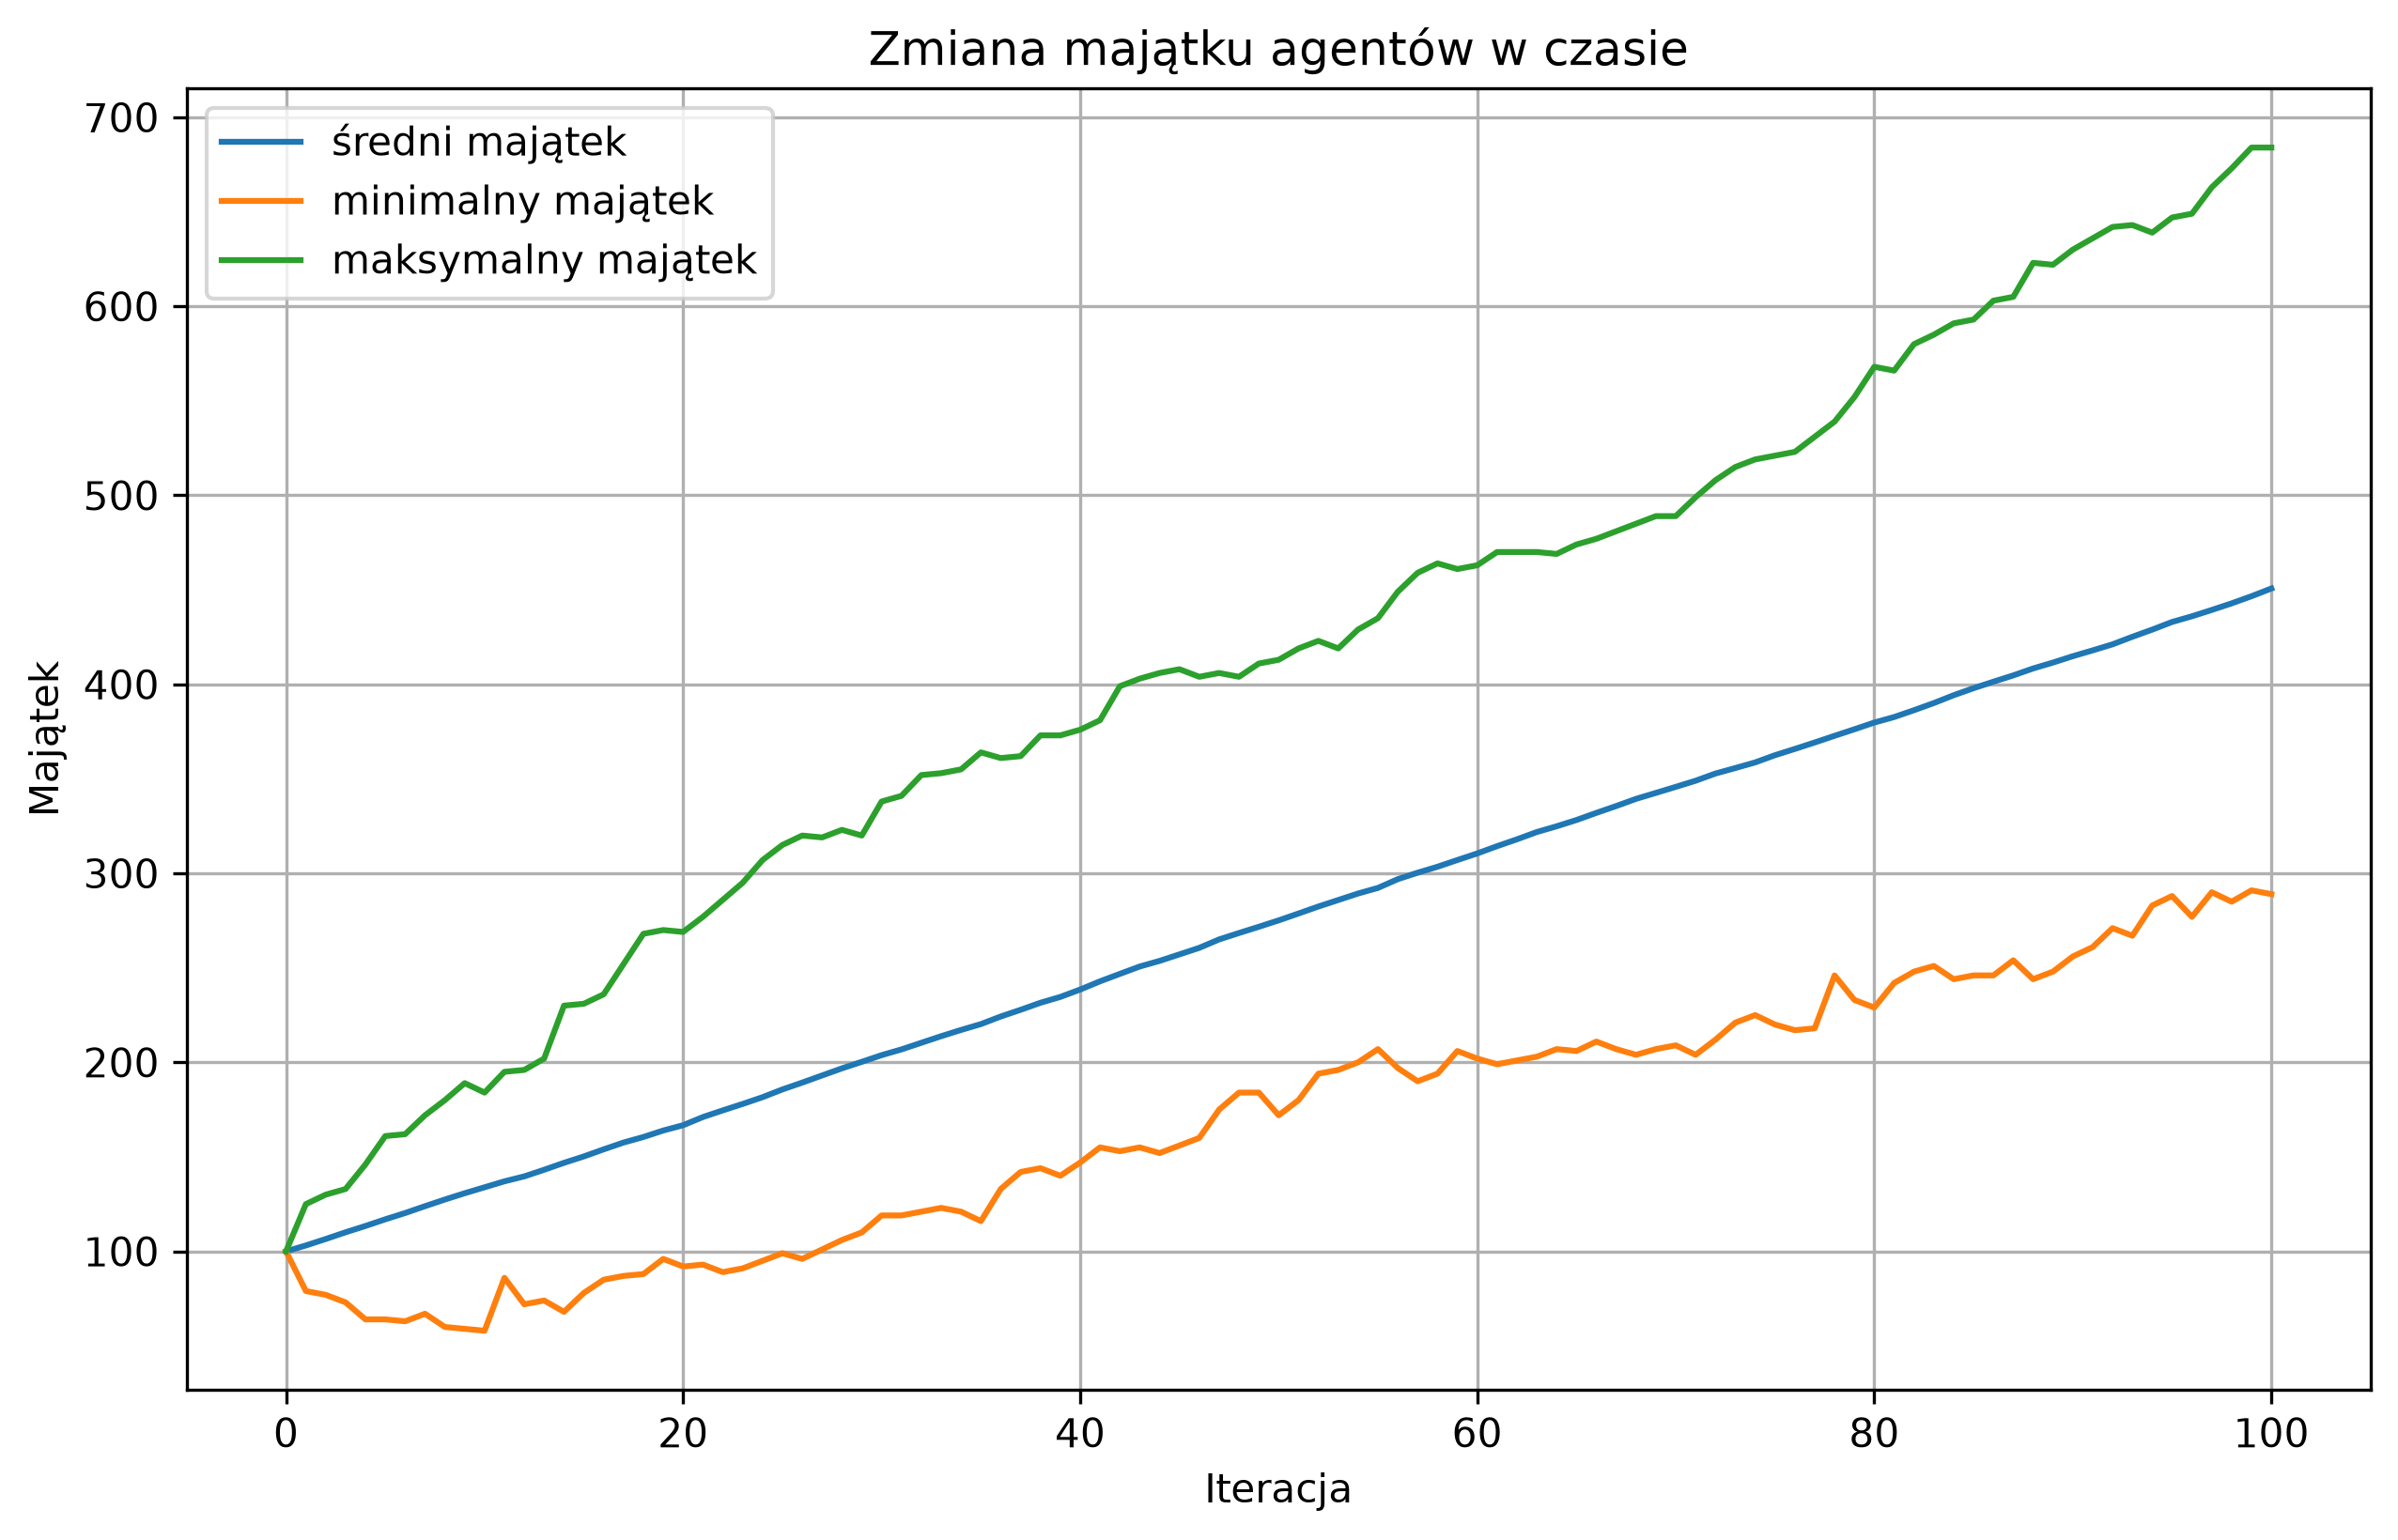
\includegraphics[width=0.8\textwidth]{figures/wealth_over_time.png}
\caption{Zmiana maj{\k a}tku agentów w czasie dla wariantu bez redystrybucji}
\label{fig:wealth_over_time}
\end{figure}

Na rysunku~\ref{fig:gini_over_time} przedstawiono zmian{\k e} wspó{\l}czynnika
Giniego w czasie dla trzech wariantów eksperymentu. Najwy{\.z}szy poziom
nierówno{\'s}ci wyst{\k a}pi{\l} w wariancie bez redystrybucji. Warianty z
redystrybucj{\k a} osi{\k a}gn{\k e}{\l}y ni{\.z}sze warto{\'s}ci wspó{\l}czynnika Giniego,
co oznacza bardziej wyrównany rozk{\l}ad maj{\k a}tku.

\begin{figure}[H]
\centering
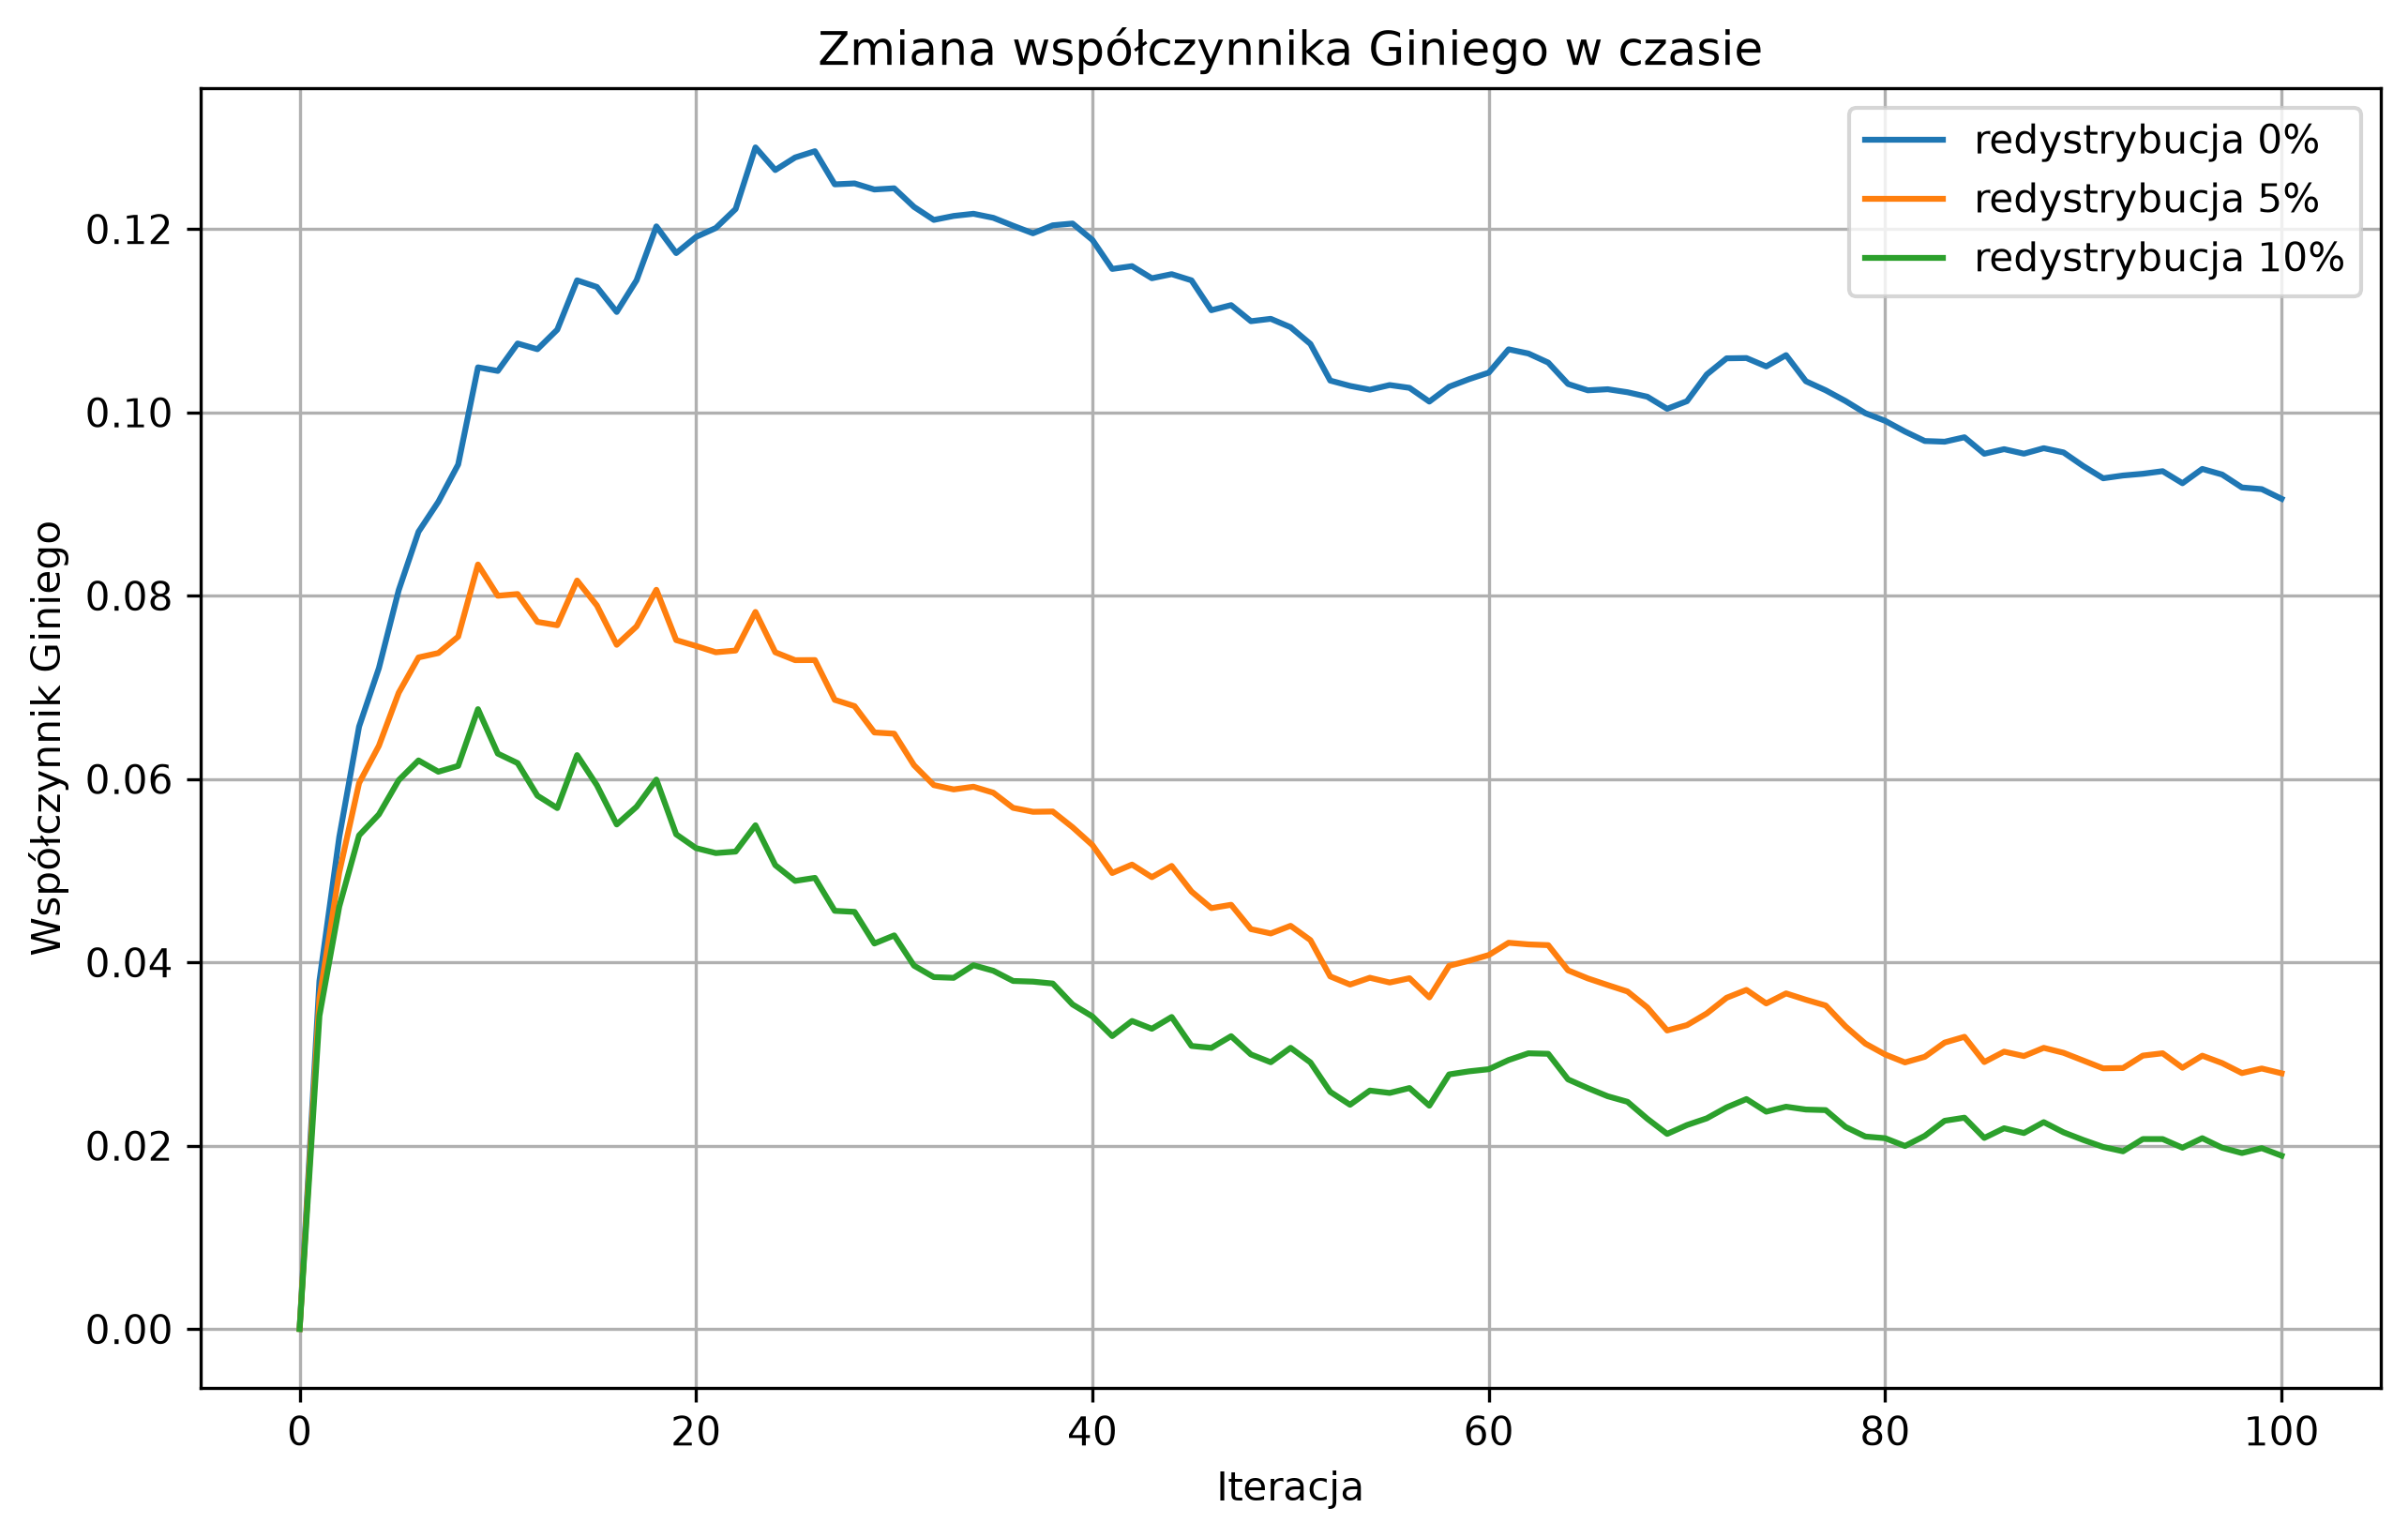
\includegraphics[width=0.8\textwidth]{figures/gini_over_time.png}
\caption{Zmiana wspó{\l}czynnika Giniego w czasie}
\label{fig:gini_over_time}
\end{figure}

Rysunek~\ref{fig:histogram} przedstawia ko{\'n}cowy rozk{\l}ad maj{\k a}tku agentów
w wariancie bez redystrybucji. Histogram pokazuje, {\.z}e po 100 iteracjach
agenci nie posiadaj{\k a} ju{\.z} takiego samego maj{\k a}tku. Cz{\k e}{\'s}{\'c} agentów
zgromadzi{\l}a wi{\k e}ksze zasoby, natomiast inni zako{\'n}czyli symulacj{\k e} z
ni{\.z}szym poziomem maj{\k a}tku.

\begin{figure}[H]
\centering
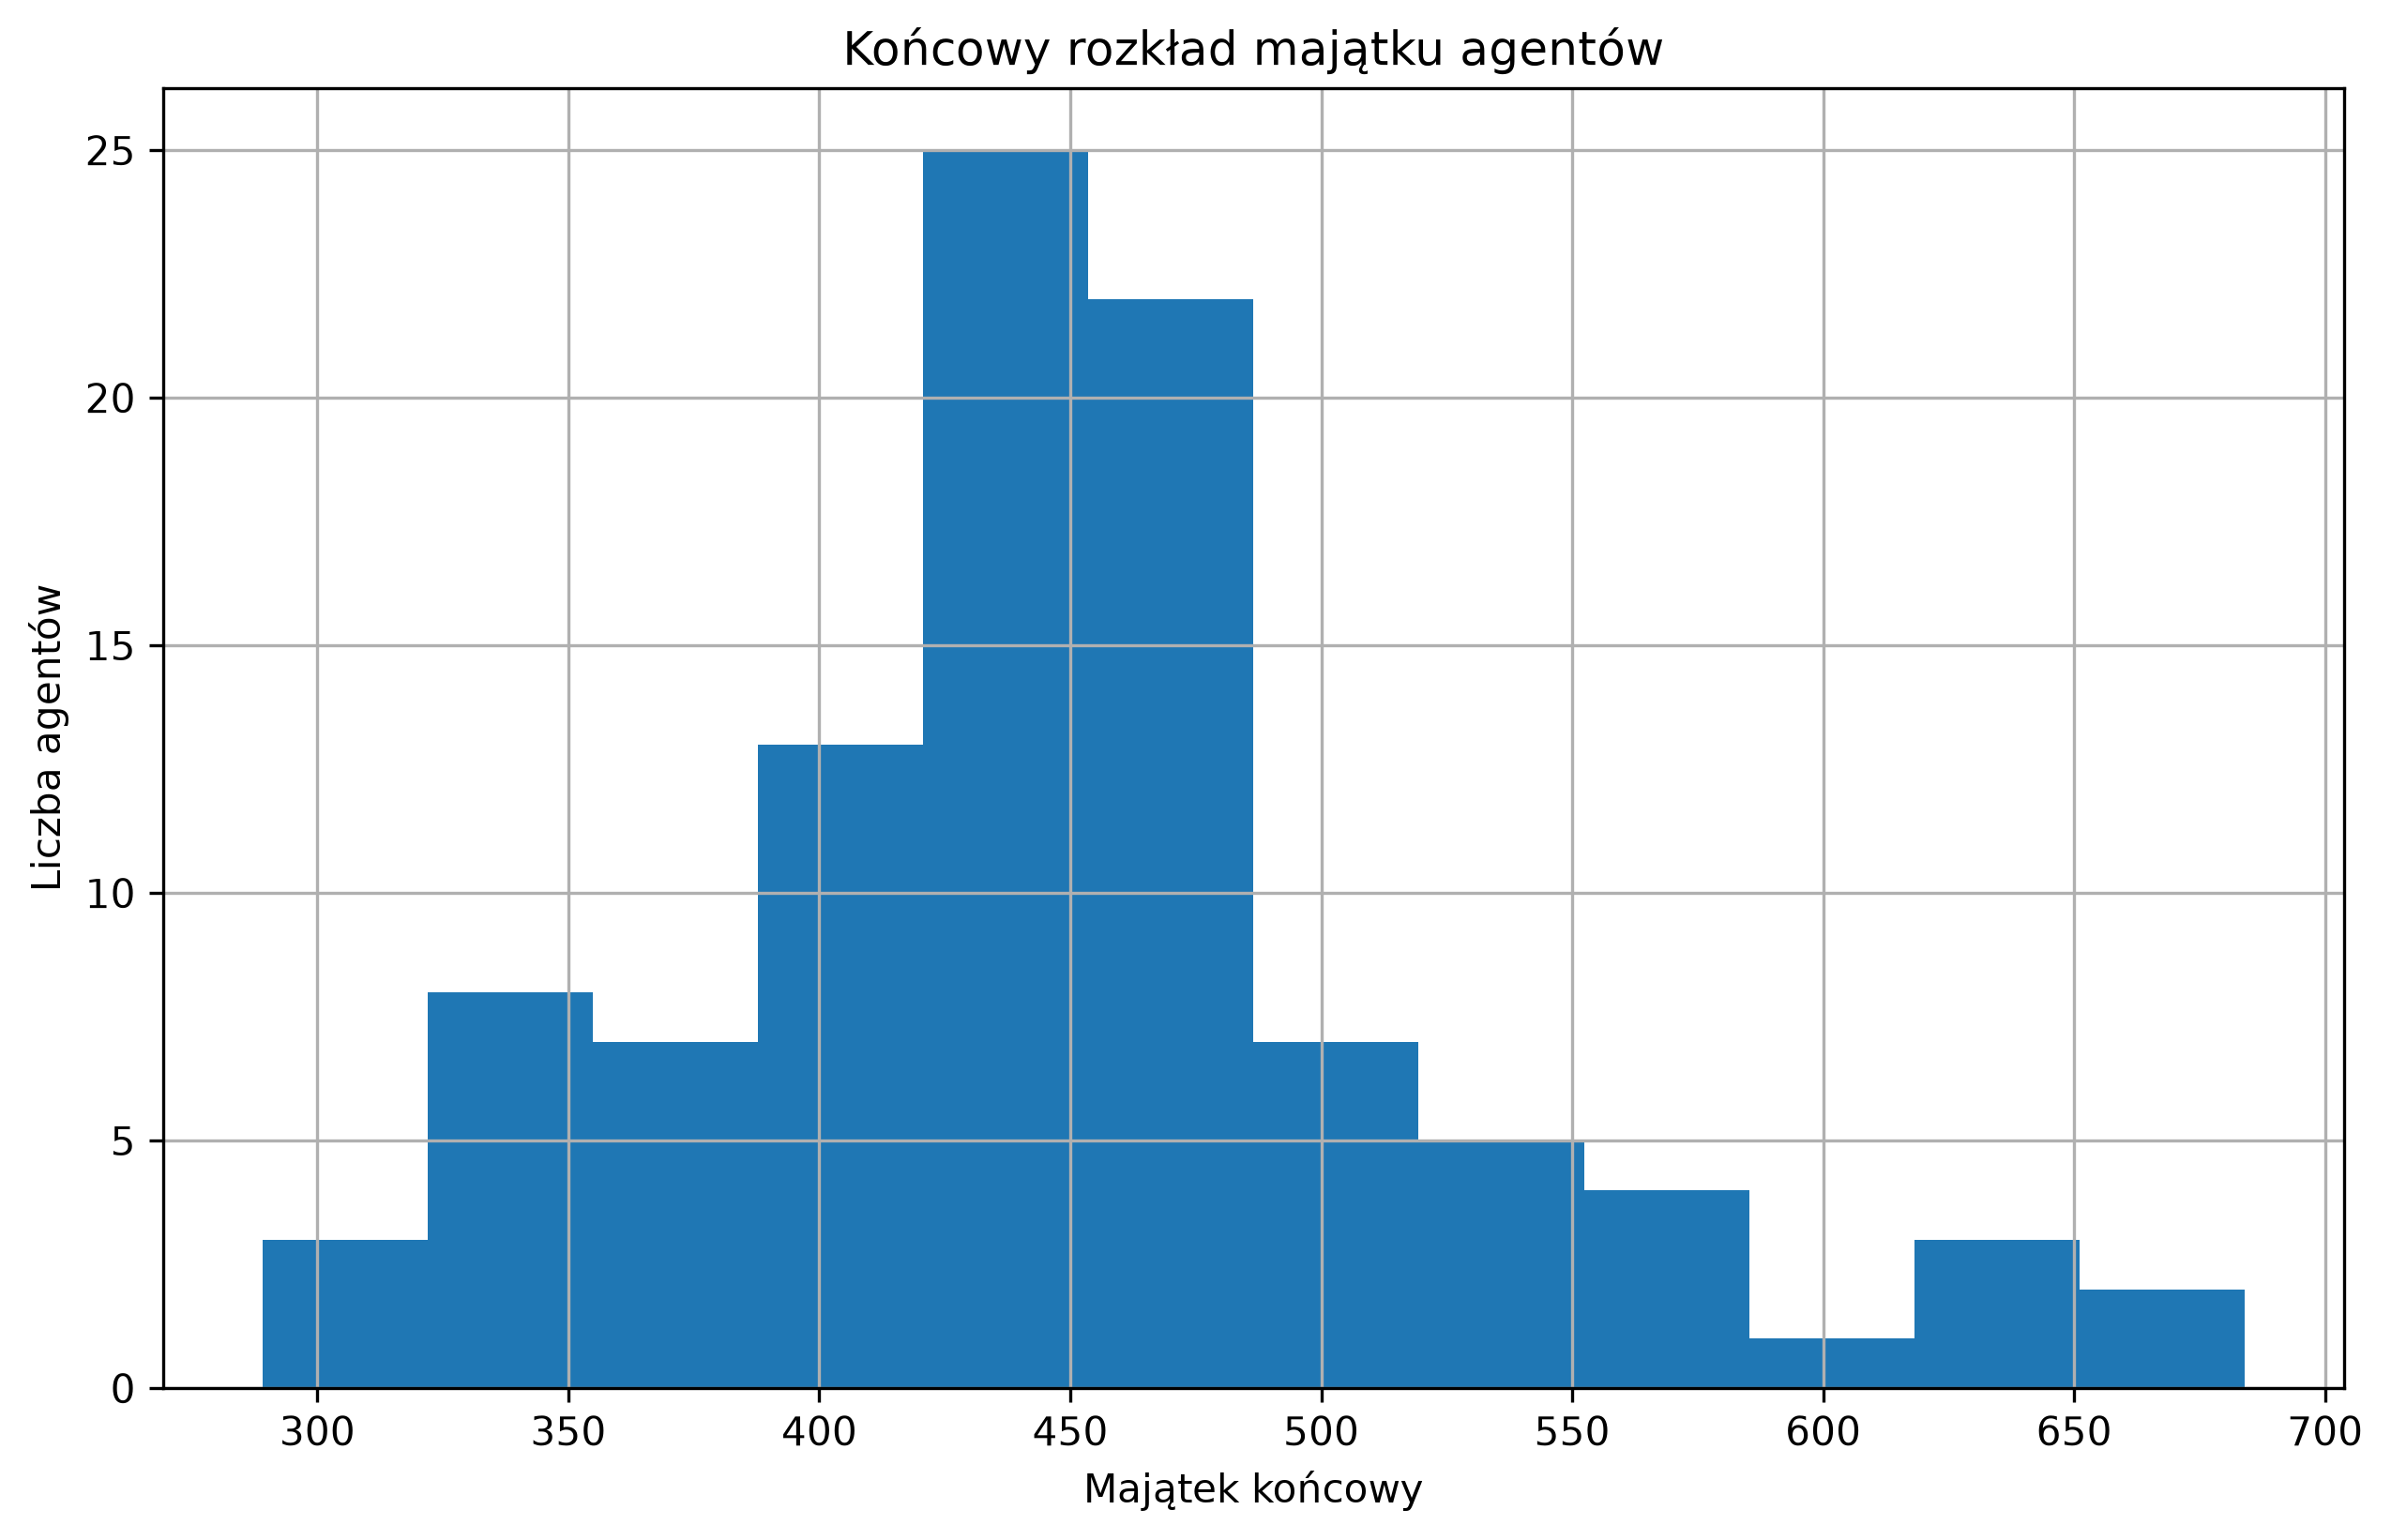
\includegraphics[width=0.8\textwidth]{figures/final_wealth_histogram.png}
\caption{Ko{\'n}cowy rozk{\l}ad maj{\k a}tku agentów bez redystrybucji}
\label{fig:histogram}
\end{figure}

\subsection{Analiza wyników}

Uzyskane wyniki potwierdzaj{\k a}, {\.z}e nawet prosty model agentowy mo{\.z}e
prowadzi{\'c} do powstawania nierówno{\'s}ci maj{\k a}tkowych. Wszyscy agenci
rozpoczynali symulacj{\k e} z identycznym maj{\k a}tkiem, jednak losowe dochody,
koszty oraz transakcje sprawi{\l}y, {\.z}e po pewnym czasie pojawi{\l}y si{\k e}
ró{\.z}nice pomi{\k e}dzy uczestnikami systemu.

Najwi{\k e}ksze nierówno{\'s}ci wyst{\k a}pi{\l}y w wariancie bez redystrybucji.
Wspó{\l}czynnik Giniego wyniós{\l} w tym przypadku 0.086. Po zastosowaniu
redystrybucji na poziomie 5\% wspó{\l}czynnik Giniego spad{\l} do 0.031, natomiast
dla redystrybucji 10\% osi{\k a}gn{\k a}{\l} warto{\'s}{\'c} 0.021. Oznacza to, {\.z}e
mechanizm redystrybucji ograniczy{\l} narastanie nierówno{\'s}ci maj{\k a}tkowych.

Wa{\.z}nym wnioskiem jest równie{\.z} to, {\.z}e redystrybucja nie zmieni{\l}a
{\'s}redniego maj{\k a}tku populacji. We wszystkich wariantach {\'s}redni maj{\k a}tek
ko{\'n}cowy wyniós{\l} 447.50 jednostek. Ró{\.z}nice dotyczy{\l}y przede wszystkim
sposobu podzia{\l}u maj{\k a}tku pomi{\k e}dzy agentów. Wariant z redystrybucj{\k a}
prowadzi{\l} do bardziej równomiernego rozk{\l}adu zasobów, natomiast wariant bez
redystrybucji sprzyja{\l} wi{\k e}kszemu rozwarstwieniu.

Przeprowadzone eksperymenty pokazuj{\k a}, {\.z}e model mo{\.z}e by{\'c}
wykorzystany do badania podstawowych mechanizmów spo{\l}eczno-ekonomicznych.
Pomimo uproszczonej struktury pozwala on obserwowa{\'c} zale{\.z}no{\'s}{\'c}
pomi{\k e}dzy lokalnymi decyzjami agentów a globalnym zachowaniem ca{\l}ego
systemu. 

%%%%%%%%%%%%%%%%%%%%%%%%%%%%%%%%%%%%%%%%%%%%%%%%%%%%%%%%%%%%%%%%%%%%%%%%%%%%%%%
\section{\SectionTitleSummary}
\label{sec:conclusions}
 
Celem pracy by\l{}o opracowanie oraz przeanalizowanie prostej symulacji systemu
spo\l{}eczno-\allowbreak ekonomicznego opartej na modelu agentowym. W~przygotowanym modelu agenci
reprezentowali uczestnik\'ow systemu ekonomicznego, kt\'orzy posiadali okre\'slony
maj\k{a}tek, uzyskiwali doch\'od, ponosili koszty \.{z}ycia oraz uczestniczyli w~losowych
transakcjach. Symulacja pozwoli\l{}a zaobserwowa\'{c}, w~jaki spos\'ob proste regu\l{}y zachowania
jednostek mog\k{a} prowadzi\'{c} do zmian widocznych na poziomie ca\l{}ej populacji.
 
Przeprowadzone eksperymenty pokaza\l{}y, \.{z}e nawet w~uproszczonym systemie, w~kt\'orym
wszyscy agenci rozpoczynaj\k{a} symulacj\k{e} z~takim samym maj\k{a}tkiem, po pewnym czasie
pojawiaj\k{a} si\k{e} r\'o\.{z}nice maj\k{a}tkowe. Wynika to z~losowego charakteru dochod\'ow, koszt\'ow
oraz transakcji pomi\k{e}dzy agentami. W~wariancie bez redystrybucji r\'o\.{z}nice pomi\k{e}dzy
najbiedniejszymi i~najbogatszymi agentami by\l{}y najwi\k{e}ksze, co by\l{}o widoczne zar\'owno
na wykresach, jak i~w~warto\'sci wsp\'o\l{}czynnika Giniego.
 
Istotnym wynikiem eksperyment\'ow by\l{}o wykazanie wp\l{}ywu redystrybucji na ograniczanie
nier\'owno\'sci maj\k{a}tkowych. Wprowadzenie redystrybucji na poziomie 5\% oraz 10\%
spowodowa\l{}o zmniejszenie rozrzutu maj\k{a}tku pomi\k{e}dzy agentami. Warto\'s\'{c} wsp\'o\l{}czynnika
Giniego by\l{}a ni\.{z}sza dla wariant\'ow z~redystrybucj\k{a}, co oznacza bardziej r\'ownomierny
podzia\l{} zasob\'ow w~populacji.
 
Wa\.{z}nym wnioskiem jest r\'ownie\.{z} to, \.{z}e redystrybucja nie zmieni\l{}a \'sredniego maj\k{a}tku
ca\l{}ej populacji. We wszystkich analizowanych wariantach \'sredni maj\k{a}tek ko\'ncowy by\l{}
taki sam. Zmianie ulega\l{} natomiast spos\'ob podzia\l{}u maj\k{a}tku pomi\k{e}dzy agent\'ow. Oznacza
to, \.{z}e mechanizm redystrybucji nie zwi\k{e}ksza\l{} ca\l{}kowitej ilo\'sci zasob\'ow w~systemie,
ale wp\l{}ywa\l{} na ich bardziej r\'ownomierne rozmieszczenie.
 
Opracowany model ma charakter uproszczony i~nie odwzorowuje w~pe\l{}ni rzeczywistej
gospodarki. Nie uwzgl\k{e}dnia mi\k{e}dzy innymi inflacji, rynku pracy, kredyt\'ow, inwestycji,
systemu bankowego ani bardziej z\l{}o\.{z}onych decyzji podejmowanych przez uczestnik\'ow
rynku. Pomimo tych ogranicze\'n model spe\l{}nia swoje zadanie, poniewa\.{z} pozwala
w~prosty spos\'ob pokaza\'{c} mechanizm powstawania nier\'owno\'sci oraz wp\l{}yw redystrybucji
na ich ograniczanie.
 
W~przysz\l{}o\'sci model mo\.{z}na rozbudowa\'{c} o~dodatkowe elementy, takie jak r\'o\.{z}ne klasy
spo\l{}eczne, zr\'o\.{z}nicowane \'zr\'od\l{}a dochodu, podatki progresywne, inwestycje, kredyty,
bezrobocie lub dziedziczenie maj\k{a}tku. Mo\.{z}liwe by\l{}oby r\'ownie\.{z} przeprowadzenie
wi\k{e}kszej liczby eksperyment\'ow dla r\'o\.{z}nych parametr\'ow oraz por\'ownanie wynik\'ow
z~bardziej zaawansowanymi modelami agentowymi opisywanymi w~literaturze.
 
Podsumowuj\k{a}c, wykonana symulacja pokazuje, \.{z}e modelowanie agentowe mo\.{z}e by\'{c}
przydatnym narz\k{e}dziem do analizy prostych system\'ow spo\l{}eczno-\allowbreak ekonomicznych.
Nawet niewielki i~uproszczony model pozwala zaobserwowa\'{c} zale\.{z}no\'s\'{c} pomi\k{e}dzy
dzia\l{}aniami pojedynczych agent\'ow a~globalnymi efektami widocznymi w~ca\l{}ym systemie.

%%%%%%%%%%%%%%%%%%%%%%%%%%%%%%%%%%%%%%%%%%%%%%%%%%%%%%%%%%%%%%%%%%%%%%%%%%%%%%%
\printbibliography

\end{document}